    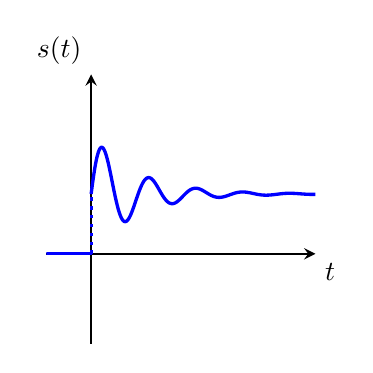
\begin{tikzpicture}
        \begin{axis}[
        axis line style = thick,
	ticks=none,
        height=5cm,
        width=5cm,
        axis x line=center,
        axis y line=center,
        xmin=-2,
        xmax=10,
        ymin=-1.5,
        ymax=3.0,
        xlabel={$t$},
        ylabel={$s(t)$},
        xlabel style={below right},
        ylabel style={above left},
        ]
        \addplot [very thick,color=blue,domain=-2:0, samples=101,unbounded coords=jump]{0};                                
	\addplot [very thick,color=blue,domain=0:10, samples=501,unbounded coords=jump]{sin(3*deg(x))*exp(-0.5*x)+1};
        \draw[dotted,very thick,blue] (axis cs:0,0) -- (axis cs:0,1); 
        \end{axis}
    \end{tikzpicture}
